
\section{Implementation}

We provide details about the nearest neighbor computation with Patch Match~\cite{Barnes09} and its multiple exemplar version Patch Web~\cite{Barnes11}.
Finally, we mention details about the different transfer strategies and especially how we got the frame disparity.

Along this section, we assume that the input frame $L'$ is the left frame and we find a k-NNF from its patches to patches within the left images $L$ of our database. The database also contains the corresponding right frames $R$ and our goal is to eventually synthesize $R'$ from $L'$.

\subsection{Patch Match}

Given an input image $A$ made of overlapping $N\times N$ patches $\{\ti\}$, we want to find the closest patches $\{\si\}$ in an image $B$, i.e.
\begin{equation}
	\si^{*} = \argmin_{\si \in B} d(\ti, \si)
\end{equation}
for some distance $d(\cdot)$, usually the sum of squared differences or a L2 norm.

A naive brute-force computation would enumerate all possible patch assignments and find the best one.
However, this is computationally unreasonnable given the context of our large high resolution image database.

Patch Match~\cite{Barnes09} is a fast approximate nearest neighbor algorithm specifically tuned for image patches and thus our problem.
It is based on the \emph{coherence assumption}, namely that, while patches mapped from $A$ to $B$ can be mapped everywhere in $B$, nearby patches in $A$ are usually mapped together in $B$.

\begin{figure}[ht]
\centering
	\begin{subfigure}[t]{0.155\textwidth}
		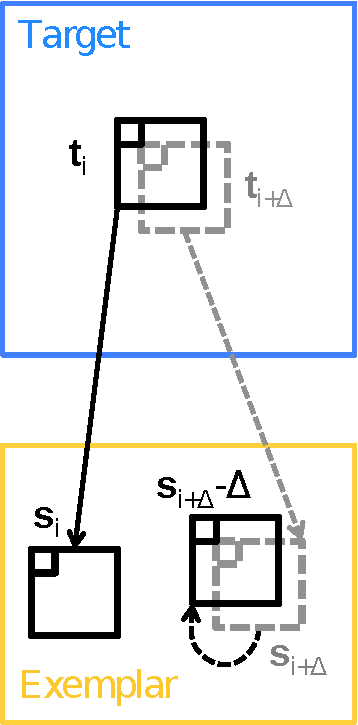
\includegraphics[width=\textwidth]{figures/propagation_text2}
		\caption{Propagation}
	\end{subfigure}
	\begin{subfigure}[t]{0.155\textwidth}
		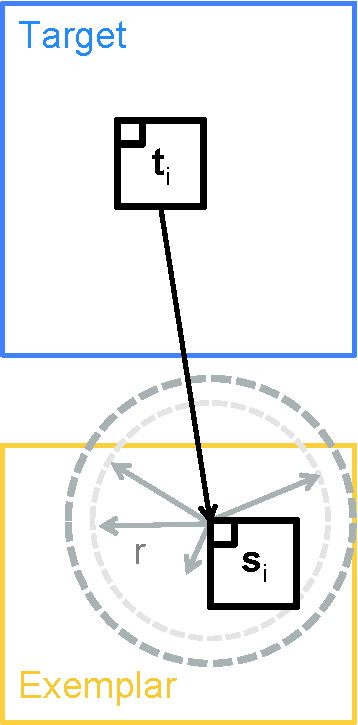
\includegraphics[width=\textwidth]{figures/randsearch_text}
		\caption{Random search}
	\end{subfigure}
	\begin{subfigure}[t]{0.155\textwidth}
		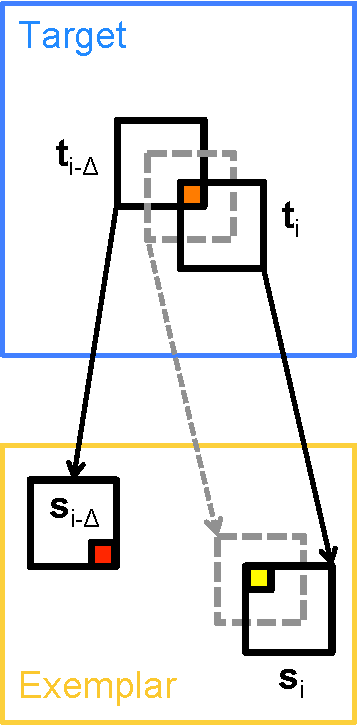
\includegraphics[width=\textwidth]{figures/voting_text}
		\caption{Voting}
	\end{subfigure}
   \caption{The main components of texture synthesis using Patch Match.}
\label{fig:texsynth_patchmatch}
\end{figure}

The algorithm proceeds in scanline-order from an initial guess of the nearest neighbor assignments $\{\ti \to \si\}$ and tries new candidate nearest neighbor patches using two main operations:
\textbf{propagation} which tries to propagate the result of neighboring mappings, and 
\textbf{random search} that randomly samples patches in an exponentially decreasing window (see illustrations in Figure~\ref{fig:texsynth_patchmatch}).

Given these patch assignments, we can transfer localized data.
This last step involves different strategies which we details in Section~\ref{sec:transfer}. 
All of them are forms of \emph{voting} since by having $N\times N$ patches, each of the pixels of our output image technically has as many overlapping patches to choose from.
The usual voting consist of averaging the overlapping pixels which minimizes the average L2 distance.

\paragraph{Extensions}
The Patch Match algorithm has been extended in several ways \cite{Barnes10} including the sampling of rotations, scales and mirrored patch spaces, the use of gain and bias adjustment, a $k$-NN version of the algorithm as well as extra operations (uniform sampling, enrichment and binning).

Application-specific variants of voting have been explored such as Meanshift \cite{Wexler07}, Histogram weighting \cite{Kopf07} as well as Bidirectional Similarity \cite{Simakov08}.

\subsection{Patch Web}
Extending the algorithm to multiple exemplars is straightforward: patches now also contain the new variable exemplar index they come from.
Furthermore, to improve performance, additional sampling strategies have been designed~\cite{Barnes11}:

\paragraph{Uniform sampling} searches over all patches of all exemplars (this is very similar to random search, with a new exemplar dimension to search through).

\paragraph{Enrichment} finds new candidates by looking at what patches we are mapped to, are mapped to (forward enrichment $f$) or to use the reverse mapping (backward enrichment $f^{-1}$) similarly.
Variants consider multiple hops such as $f^2$, $f^3$, $\dots$ or $f^{-2}$, etc.

Given a $k$-NNF, one can use enrichment with the $k$ candidates or a subset, leading to many potential variants.

\paragraph{Binning} divides the patches into bins similarly to what a histogram would do, and samples patches from the bin corresponding to the patch we sampling for.
To bin patches, usually a lower-dimension space is used ($N\times N$ patches with $C$ channels have $CN^2$ dimensions) by computing PCA.

Recent alternatives~\cite{He12} use Walsh-Hadamard Transform bases~\cite{Hel05} instead of PCA.

Our implementation contains all the aforementioned candidate lookups but binning because of the high memory requirement that makes it harder to implement wisely (other strategies require basically no additional memory storage).

\subsection{Stereo Transfer}
\label{sec:transfer}
Armed with an effective multiple exemplar k-NNF computation, there remains to transfer the stereoscopic information and synthesize our right frame.

\begin{enumerate}
	\item Compute constrained k-NNF from left to right
	\item Vote disparity
\end{enumerate}

Multiple voting strategies are possible:
\begin{itemize}
	\item Merge k-NNF into 1-NNF and then take naive patch shift as disparity
	\item Compute average disparity of $k \times N \times N$ overlapping patches
	\item Compute it with Mean-Shift
\end{itemize}

\TODO{Use patches with 5 channels: L, a, b, x, y}
\TODO{location of patch matters for disparity}

\TODO{talk about the missing "binning"}

\TODO{mention halfway domain}